% !TEX root = ../thesis.tex
\chapter{Web application - BotBuster}
\label{capitolo6}
\thispagestyle{empty}
This chapter represents the practical application of our work. We wanted to provide a tangible proof the thesis, an instrument available to every users in search of classification, among the accounts met on Twitter.
We thought it was useful to allow people to be aware about the nature of the users that populate the social network.
Bots often don't claim themselves as automated accounts, that makes hard their detection, even for an experienced utilizer.


\textbf{BotBuster} is the name of the project, whose goal is to provide the probability-based classification of the desired Twitter user.
The probabilities are shown in a histogram-shaped graph, with different colours, one for each target, as displayed in Figure\ref{fig:histogram}.

\begin{figure}
	\begin{center}
		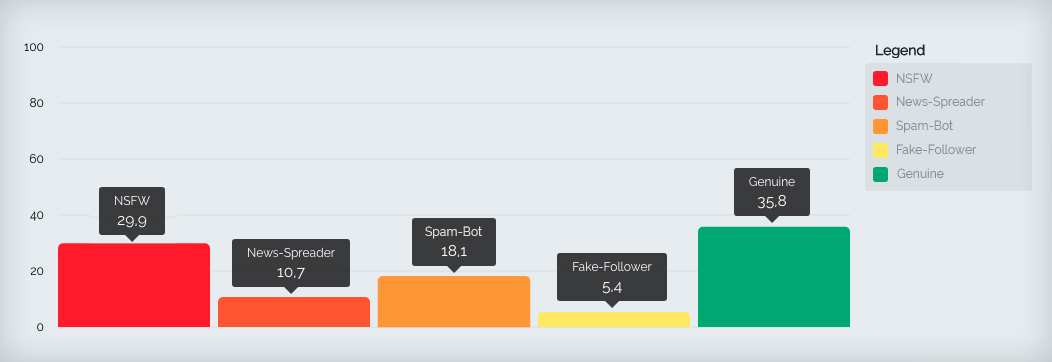
\includegraphics[width=\columnwidth]{chapter6/figure/histogram.jpg}\par 
	\end{center}
	\caption{Probability classification diagram on BotBuster}
	\label{fig:histogram}
\end{figure}

The web application had to be visible on a public URL. It is currently available on \href{http://www.botbuster.it}{\textit{www.botbuster.it}}.

Basically, the functioning of BotBuster can be resumed in getting a Twitter user name through an input filed on the home page, and then executing the prediction pipeline described in chapter \ref{predicion_pipeline}.
The input filed filling triggers the engine operating in the background, which runs a Python script performing the prediction.
\section{Architecture}
The web application works under a client - server paradigm. The Angular program is executed on the client's web browser, while on the server runs the Flask application.
Every time a user search for a Twitter user name, the HTTP protocols is involved to perform POST and GET requests between client and server. The frontend and the backend applications handle the request and exchange, as shown in Figure\ref{fig:architecture}.
\begin{figure}
	\begin{center}
		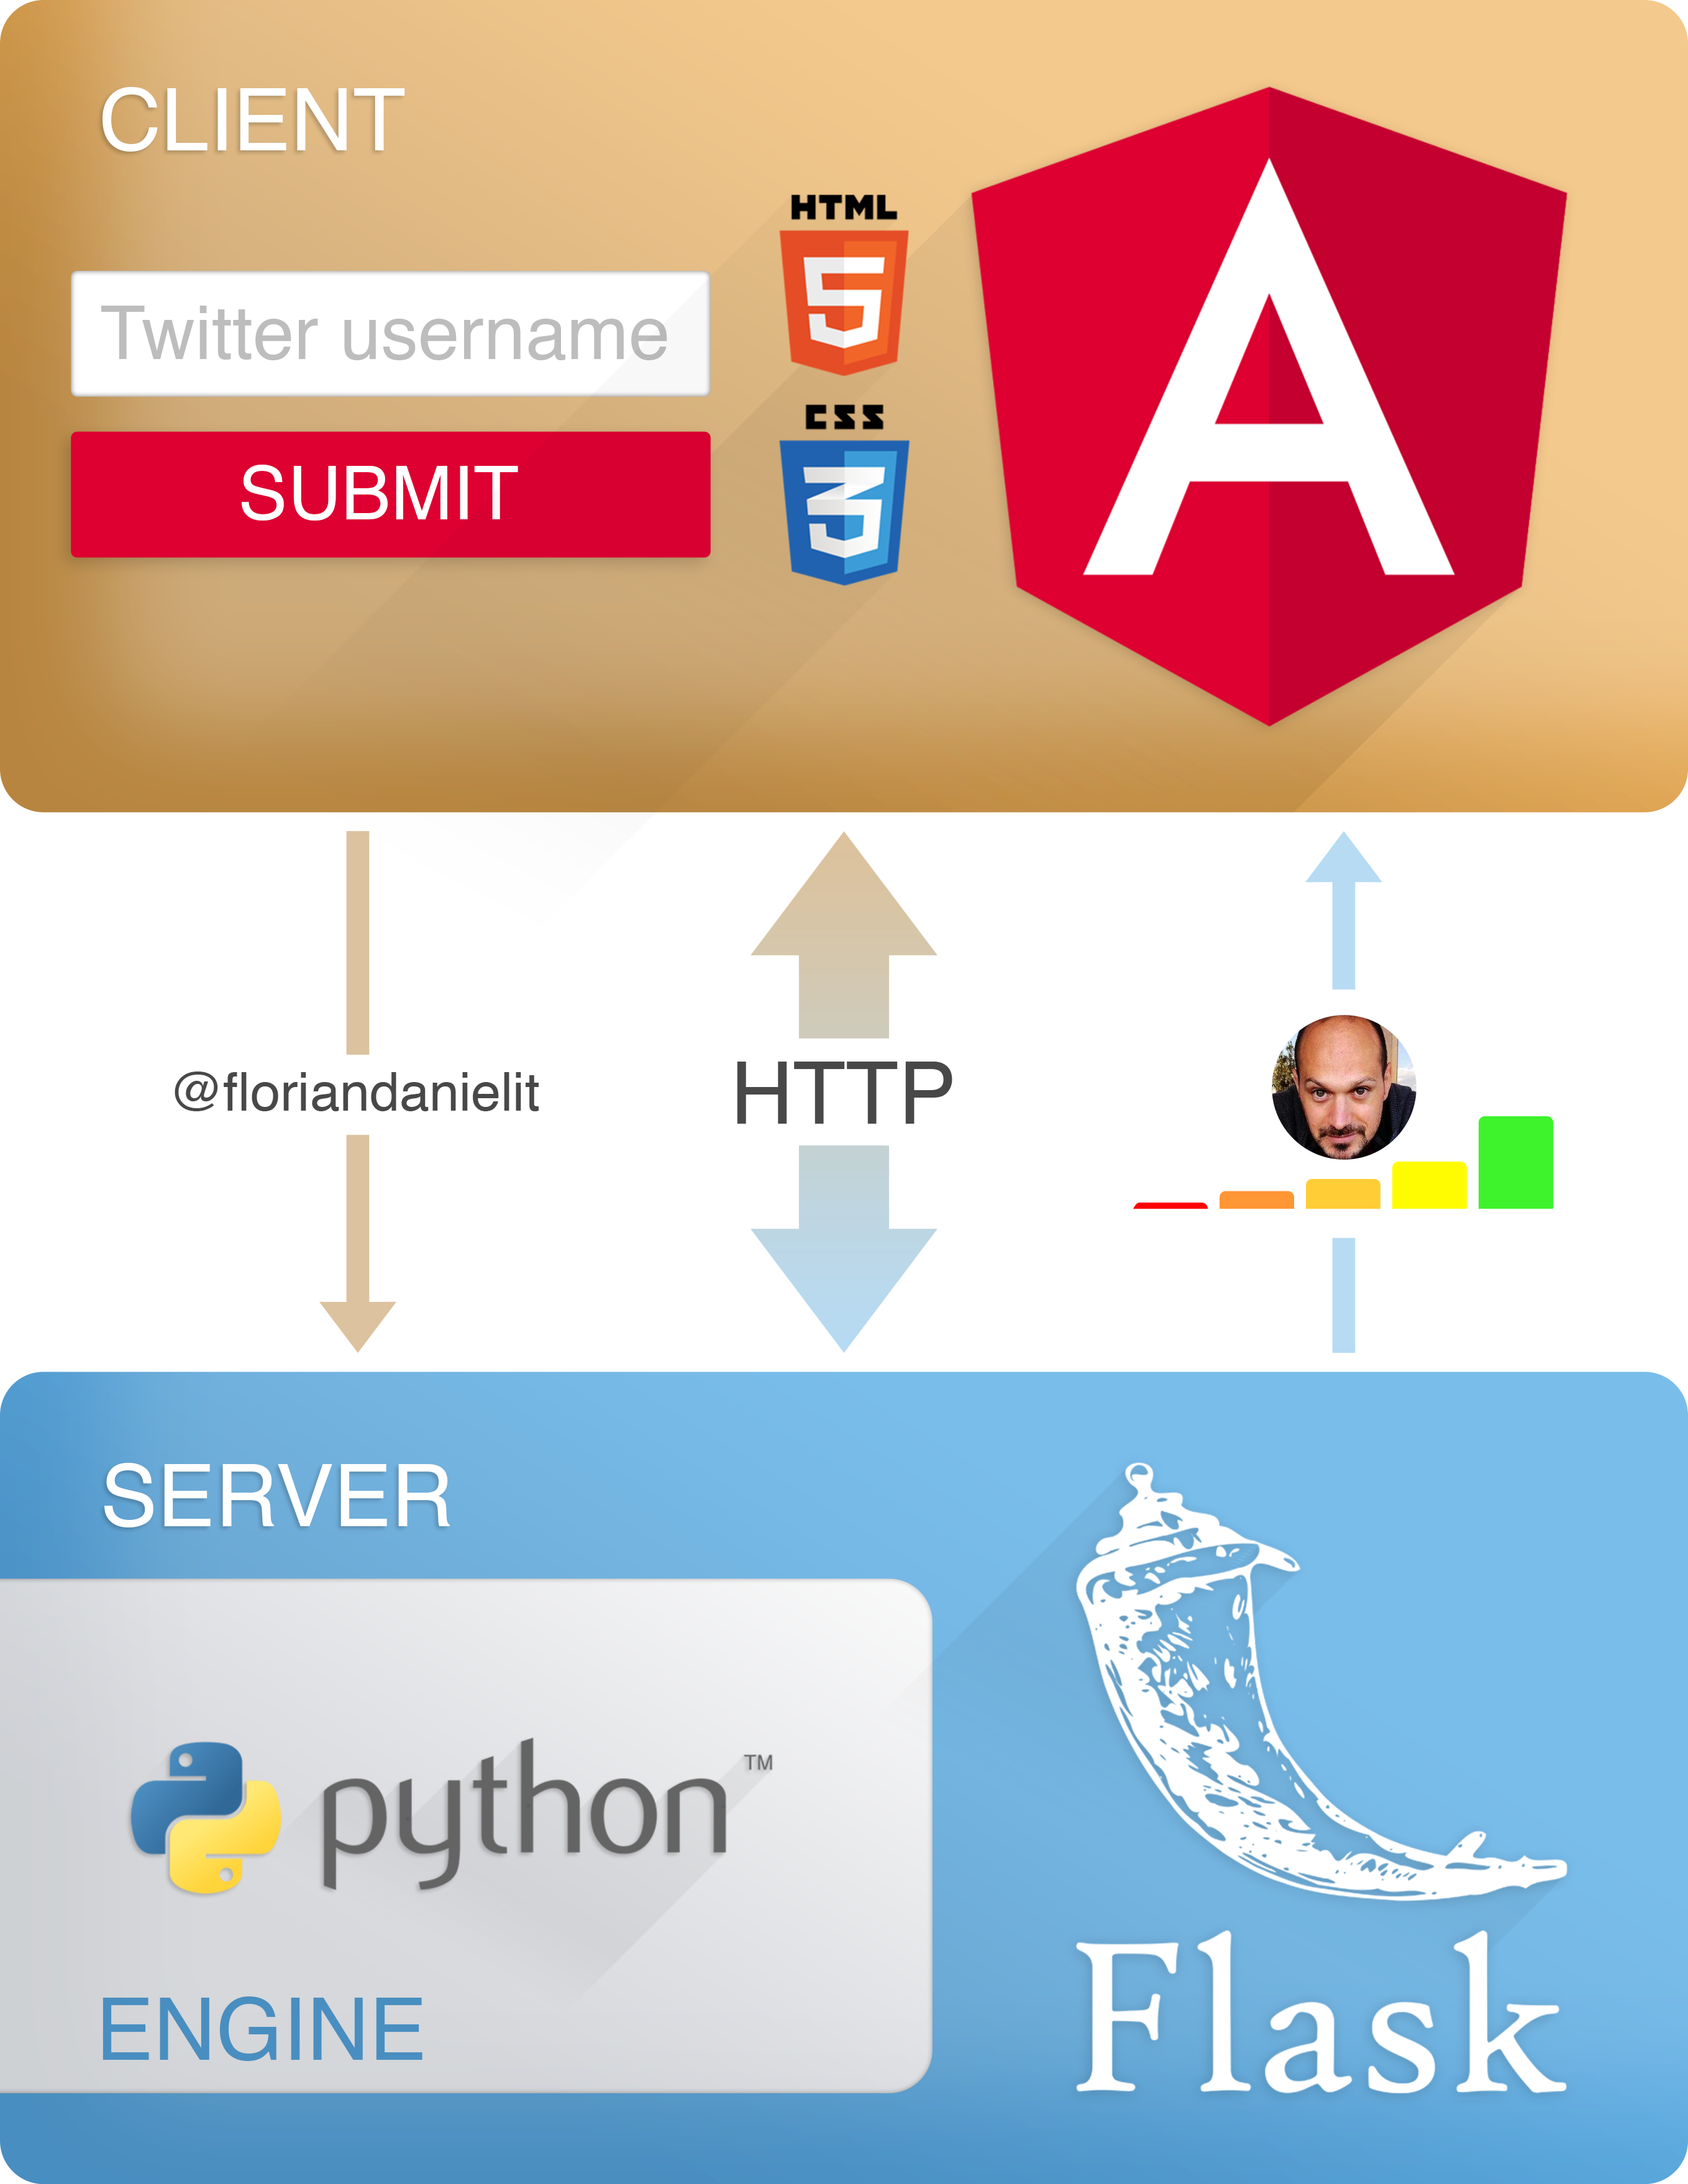
\includegraphics[width=0.6\columnwidth]{chapter6/figure/architecture.png}\par 
	\end{center}
	\caption{Client - Server architecture}
	\label{fig:architecture}
\end{figure}

\section{Backend}
\subsection{Engine}
The real engine of the web application is a Python 3 script. It performs all the steps described in the pipeline execution section \ref{predicion_pipeline}.
The models, that have been previously fitted with data, serialized and stored, are now loaded by the Python script. They have to perform a single prediction at a time.
In addition to the models we built for the classification, the pre-trained convolutional neural network for NSFW recognition has been introduced to the pipeline, in order to infer on the media contents posted by the examined user.
The first step consists in calling the Twitter APIs to retrieve user's data and its most recent tweets, up to 100. 
The script, then, handles the preprocessing stages and the data preparations needed by the different classifiers.
Two final predictions are computed: the binary and the mutliclass classification.
The probability given to the bot target, by the binary classifier, is used to weight the mutliclass prediction provided by the stacking ensemble.
The final classification is composed by five probabilities: \textbf{P\textsubscript{NSWF},} \textbf{P\textsubscript{News-Spreader}}, \textbf{P\textsubscript{Spam-Bot}}, \textbf{P\textsubscript{Fake-Followers}}, \textbf{P\textsubscript{Genuine}}.
\subsection{Flask}
\section{Frontend}
\section{Deployment platform}
\section{Validation}
